\subsection{Insert and update using the \texttt{upsert}-function}\label{subsec_upsert_data_function}

Suppose you have created a CSV table with, say, cabinet configuration that contains both new cabinet configurations and, in addition, changes to already existing cabinets. That is, the listed cabinet configurations in your table may match some recorded cabinet configurations in the PCDB cabinet table. 

Due to the \texttt{UNIQUE}-constraint on \texttt{ctr\_id} and \texttt{cab\_sdate} in the cabinet table, attempting to insert cabinet configurations that are identified by an already recorded \texttt{ctr\_id}-\texttt{cab\_sdate} combination would prompt an error. 
And its likely that, while you want to add not-yet recorded configurations to the cabinet table, you simply want to update the already existing configuration in the PCDB where the information on a given configuration on in your table differs from that in the current record.
This scenario is where the \texttt{upsert}-function comes in to play (`upsert' stands for update-or-insert).

Plainly speaking, the \texttt{upsert}-function performs exactly the steps outlined in the above paragraph: 
First, it takes your table as source of the upsert operation, checking which columns actually correspond to the columns of the target table (i.e., the table you want to populate with your new records). 
Second, the function checks if a record in the source table matches a record (i.e., row) in the target table.
The result of this second step are two distinct result sets (your source table is split into two categories, so to speak): One containing all observations that are not yet recorded in the target table. This first result set is the base of a grand insert operation on the target table.
The other result set comprises all observations in the source table that are already recorded in the target table, and hence is the base of a grand update opertion on the target table. 

Put simply, the function looks up which column(s) contain the primary key of the target variable, and then checks if a given observation's primary-key column value in the source table exists in the target table. 
For example, \texttt{cab\_id} is the primary-key column of the cabinet table. Say your target table contains a cabinet configration with the \texttt{cab\_id} value 1040.
If `Is 1040 is in the list of all values of the \texttt{cab\_id} column in target table?' evaluates to true, this row in the source table will be in the second result set. 
Otherwise it will be in the first, insert-operations result set.


\subsubsection{Function description}

Because the \texttt{upsert}-function is at the heart of the updating process, it follows a detailed description of its working in verbatim pseudo-code.

You may want to skip this paragraph if you are immediately interested in a minimal working example (beginning on page \pageref{par_upsert_minimal_working_example}). 
You may need to turn to the functional defintion, however, Whenever the \texttt{upsert}-function is not yielding the results you were intending it to give.

Function \texttt{upsert\_base\_table()} is defined in the \texttt{public} schema of the \texttt{polconfdb} database.%(Lines 3-5) 
\begin{itemize}
\item[-]{It has four input arguments:
  \begin{itemize}
  \item[-]{\texttt{target\_schema}: schema name of the table that is upserted (target)}
  \item[-]{\texttt{target\_table}: name of the table that is upserted (target)}
  \item[-]{\texttt{source\_schema}: schema name of the table that is the source of the upserted operation}
  \item[-]{\texttt{source\_table}: name of the table that is the source of the upserted operation}
  \end{itemize}
All input arguments have require type \texttt{TEXT}.
}
\item[-]{Return type is \texttt{VOID}, i.e., nothing is returned}
\item[-]{\texttt{DECLARE} variables that will be used in \texttt{EXECUTE} block:%(lines 48-69)
\begin{itemize}
  \item[-]{variable \texttt{pkey\_column} stores the name of the column that contains the primary key of the target table}%(Lines 9-12)
  \item[-]{variable \texttt{pkey\_constraint} stores the name of the primary key constraints of the target table}%(Lines 14-17)
  \item[-]{array \texttt{shared\_columns} stores a comma-seperated list of the columns the target and source tables have in common; will be used in \texttt{INSERT}-statement%(lines 58 and 59)
  }%(Lines 19-30)
  \item[-]{array \texttt{update\_columns} stores a comma-seperated list of target columns that are set equal to source columns in \texttt{SET}-statementto of update operation%(line 50)
  }%(Lines 32-46)
\end{itemize}
}%(Line 8 ff.)
\item[-]{\texttt{EXECUTE} block:%(Lines 48 ff.)
\begin{itemize}
    \item[-]{execute \texttt{UPDATE} of target table, setting target column values equal to source column values for all intersecting identifiers% (\texttt{WHERE}-clause, lines 52-54)
    }%(Lines 49-56)
    \item[-]{execute \texttt{INSERT INTO} target table, inserting data into from source table for all rows that are not in target table (set difference of identifiers)}%(Lines 58-64)
    \item[-]{cluster data, i.e., order by priamary key values}%(Line 66)
\end{itemize}
}
\end{itemize}
A definition of function \texttt{upsert\_base\_table()} in the \texttt{PostreSQL} procedural language \texttt{plpgsql}\footnote{See \url{https://www.postgresql.org/docs/8.4/static/plpgsql.html}} is provided in the Appendix (see \ref{subsec_appx_fun_upsert_base_table}).

\subsubsection{A minimal working example}\label{par_upsert_minimal_working_example}

To stick with the above example of making changes to the cabinet table in the PCDB, suppose yout task is to check cabinet start dates, and to add cabinet configurations that are not yet recorded in the \texttt{config\_data} schema of the database.
Say you split the work load with your co-workers, and you start with checking and updating all Australian cabinet configurations.

\paragraph{Exporting the to-be-updated data}
The first step in a well-organized work flow would be to export all recorded Australian cabinet configurations that require a double-check of the start date into a CSV.
The following query would give you just these configurations: 
\begin{lstlisting}[language=postgreSQL]
SELECT * FROM config_data.cabinet 
	WHERE ctr_id = 1
	AND cab_valid_sdate = FALSE;
\end{lstlisting}
Note that the column \texttt{cab\_valid\_sdate} is a boolean indicator that records whether the start date of a given cabinet configuration has already been double-checked. Hence, you only want the Australian cabinet configurations where this is not yet the case.

Exporting the result set of the query int o a CSV is easily achieved using the write-result-to-file wizard of \texttt{pgAdmin3}'s SQL-query tool. (Refer to Subsection \ref{subsec_sql_query_tool}, and figures \ref{fig_pgadmin3_sql_query_tool_toolbar} and \ref{fig_pgadmin3_sql_query_tool_export_data_wizard} in particular, if you do not know how to do export data to a file in \texttt{pgAdmin3}.)

In order to know which Australian cabinets are not yet recorded, and hence need to be added in your `upsert' source table, you need to know, which is the youngest recorded Austrian cabinet in the PCDB (i.e., the cabinet with the most recent start date). 
the The result set of the above query does not necessarily inform you about this,  however (if \texttt{cab\_valid\_sdate} is true for the last recorded cabinet configratuion, it will not be in the result set.)

You could query 
\begin{lstlisting}[language=postgreSQL]
SELECT * FROM config_data.cabinet 
	WHERE ctr_id = 1
	ORDER BY cab_sdate DESC
	LIMIT 1;
\end{lstlisting}
in order to get the respective information, or export all Austrian cabinet configurations in the first place, and only check start dates of these where  \texttt{cab\_valid\_sdate} is false instead.

\paragraph{Changing the to-be-updated data}
With the exported CSV at hand, you can directly make your changes in the repective cells of the table; of course always documenting your changes and the information sources in the comment and source columns.
In case of already existing cabinets, you would not change the \texttt{cab\_id} but only the \texttt{cab\_sdate}.
In case of missing cabinets, you would choose a not existing \texttt{cab\_id} value (optimally increasing it by one within country with ascending start dates) and add all corresponding inforamtion in the respective cells of that new entry.

\paragraph{Getting the to-be-updated data into the PCDB}
In order to upsert the target table with the changes you have recorded in your CSV, the data in your CSV first needs to be imported into the PCDB again.
The \texttt{updates} schema of the PCDB provides for the environment in which you can securely import to-be-updated data into upsert source tables.

Note that, if it not already exists, you first have to create a table in the \texttt{updates} schema that matches the column names and types of your CSV.
If you have proceeded as described thus far in this minimal working example, your CSV containing the to-be-updated data will have the same definition as the upsert target table (because the CSV was orginally exported from the target table).
Hence you can simply type 
\begin{lstlisting}[language=postgreSQL]
CREATE TABLE IF NOT EXISTS updates.cabinet (LIKE config_data.cabinet INCLUDING ALL)
\end{lstlisting}
Note that the option \texttt{INCLUDING ALL} will create a new table that copies all column names, their data types, their not-null constraints, primary and foreign key.\footnote{See \url{https://www.postgresql.org/docs/9.1/static/sql-createtable.html}}
The resulting table will be empty but prompt the same requirments when inserting data as the target table (here cabinet in the \texttt{config\_data} schema). 
That is, you won't be able to insert duplicate \texttt{cab\_id}s, rows with missing start date information, etc. (see the definition of table cabinet for a compelte list of column and table cosntraints).

Once you have created an empty source table in the \texttt{updates} schema as, you can use \texttt{pgAdmin3}'s easy-to-handle import wizard to import data to the now existing table.\footnote{%
If the table is not empty, e.g., storing data from previous updating rounds, its recommended to remove the superflous data before adding new to-be-updated data. 
Use the `Drop/Delete ...' function provided on right-click on the respective table in the Objecet Browser or explicit SQL to empty the source table.}
Simply right-click on the table in the Object Browser and select ``Import'' (See Figure \ref{fig_pgadmin3_import_data_to_table}). 
The `Import data from file into table' wizard will open (shown for the case of the cabinet table in Figure \ref{fig_pgadmin3_import_data_wizard_file_options}), and allow you to browse your system for the respective CSV. 
Remember to select check-box `Header' in the `Misc. Options' tab of the wizard and enter the delimiter of the data (see Figure \ref{fig_pgadmin3_import_data_wizard_misc_options}).\footnote{In CSVs produced with German default settings, columns are usually separated with semicolons (\texttt{;}).}

\begin{figure}[ht!]
\centering
  \begin{subfigure}{.50\textwidth}
  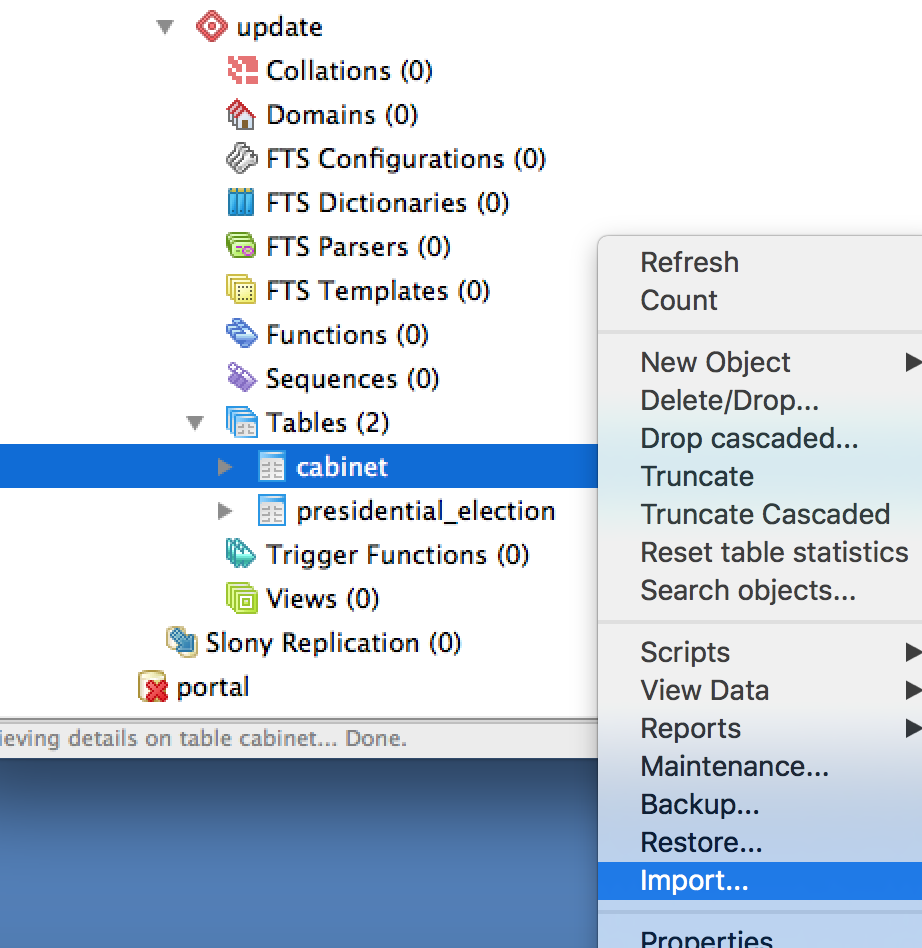
\includegraphics[width=\textwidth,trim= 0 0 0 0, clip]{pcdb_documentation_screenshots/pgadmin3_import_data_to_table.png}
    \subcaption{How to open the data-import wizard for a table in \texttt{pgAdmin3}'s Object Browser.}
    \label{fig_pgadmin3_import_data_to_table}
  \end{subfigure}
  ~%
  \begin{subfigure}{.40\textwidth}
    \begin{subfigure}{1\linewidth}
    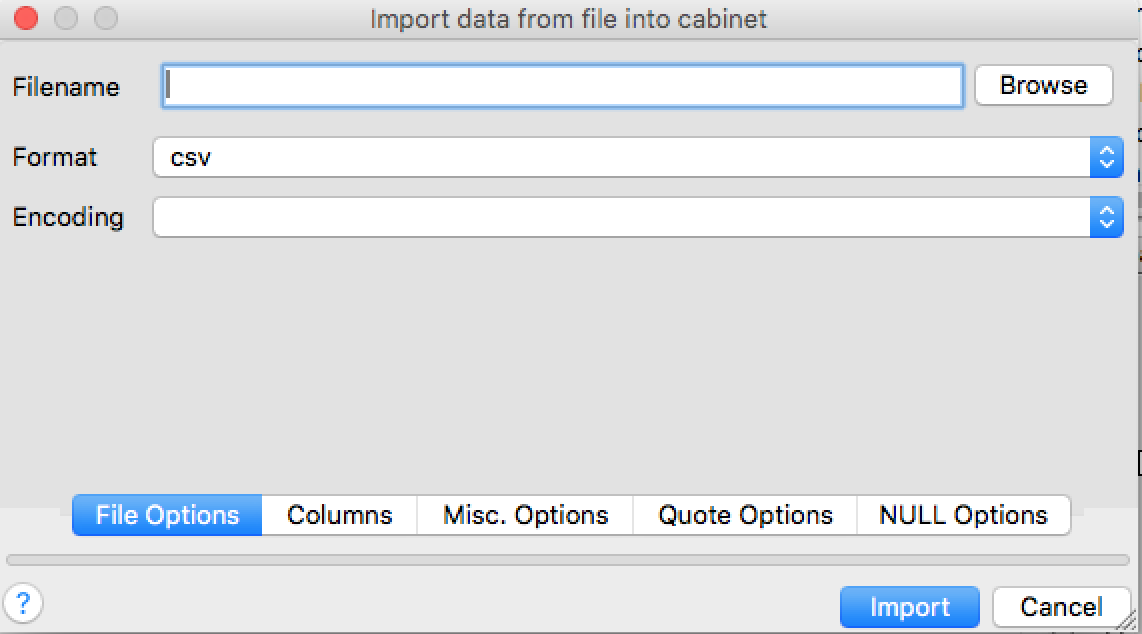
\includegraphics[width=\textwidth,trim= 0 0 0 0, clip]{pcdb_documentation_screenshots/pgadmin3_import_data_wizard_file_options.png}
      \subcaption{The `File Options' tab.}
      \label{fig_pgadmin3_import_data_wizard_file_options}
    \end{subfigure}
    ~\\%
    \begin{subfigure}{1\linewidth}
    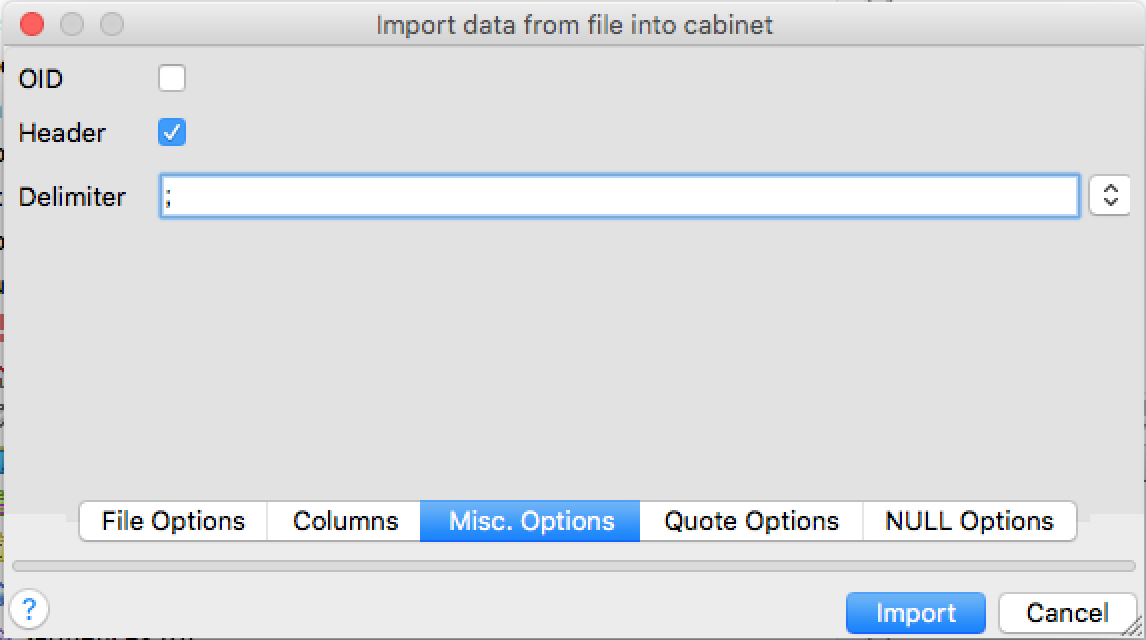
\includegraphics[width=\textwidth,trim= 0 0 0 0, clip]{pcdb_documentation_screenshots/pgadmin3_import_data_wizard_misc_options.png}
      \subcaption{The `Misc. Options' tab.}
      \label{fig_pgadmin3_import_data_wizard_misc_options}
    \end{subfigure}
  \end{subfigure}
\caption{\texttt{pgAdmin3}'s `Import data from file into table' wizard.}
\end{figure}

In case you have initially exported fewer columns from the target table, you can use the `Columns' tab in the wizard to unselect the columns of the source table that are not recorded in your CSV.

Alternatively, you can define a table writing explicit SQL. 
Suppose, for instance, you have updated presidency start dates (i.e., column \texttt{prs\_sdate}) for configurations in table presidential election, but your work-in-progress CSV looks like the example displayed in Figure \ref{fig_excel_update_prs_sdate_csv}.

\begin{figure}[ht!]
  \centering
  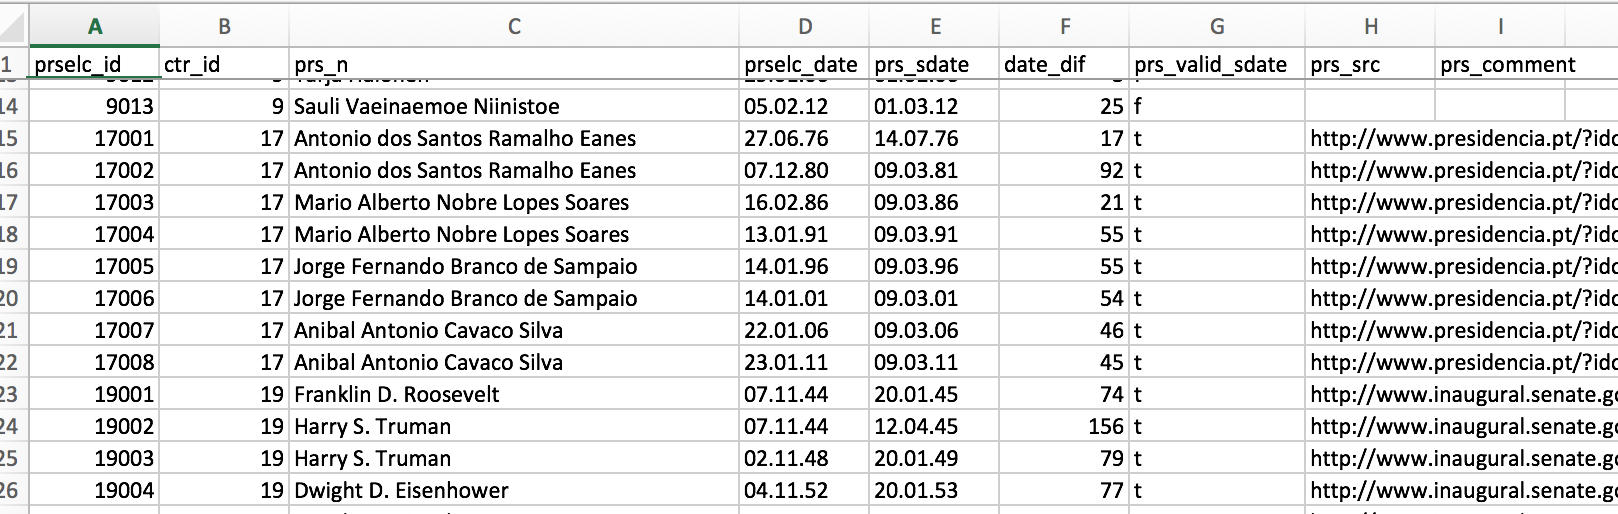
\includegraphics[width=0.9\textwidth,trim= 0 0 0 0, clip]{pcdb_documentation_screenshots/excel_update_prs_sdate_csv.png}
  \caption{Example of CSV with to-be-updated data that does not match column structure of target table.}
  \label{fig_excel_update_prs_sdate_csv}
\end{figure}

Because the order of the columns in this CSV do not match the order of columns in the target table (e.g., in the CSV \texttt{prs\_n} comes before \texttt{prselc\_date} and \texttt{prs\_sdate}, whereas it comes between \texttt{prselc\_date} and \texttt{prs\_sdate} in the target table), just unselecting the columns that do not exist in the source table when importing data to an exact, empty copy of the presidential election table in the \texttt{updates} schema would nor fix the problem.
Instead, you would have to define a matching table in the \texttt{updates} schema like
\begin{lstlisting}[language=postgreSQL]
CREATE TABLE updates.presidential_election (
	prselc_id	NUMERIC(5,0)	PRIMARY KEY	,
	ctr_id		SMALLINT	UNIQUE NOT NULL,
	prs_n		NAME	, 
	prselc_date	DATE	UNIQUE NOT NULL,
	prs_sdate	DATE	, 
	date_dif	INTEGER	,
	prs_valid_sdate	BOOLEAN	,
	prs_src		TEXT	, 
	prs_comment	TEXT);
\end{lstlisting}

The work-flow in this example is clearly more complicated, so be aware of the difficulties arising from non-matching column ordering when attempting to update an existing table in the \texttt{config\_data} schema.\footnote{You may wonder why then deviating from the column structure of the target table should be considered at all when creating (i.e., exporting) a CSV with to-be-updated data. 
The answer is readability. Some tables, like the lower house election tables have more then a dozen of columns; just exporting the data from the columns that actually require updating then is quiet convenient. And you are on the sage side, if you simple stick to the column order in the target table.}
%Refer to section \ref{sec_tables} for examples. 

\paragraph{Upserting the target table based on the data in the source table}
Let'S return to our previous minimal workin example: updating the cabinet table.
Once you have exported the to-be-updated data from your target table into a CSV, made your changes in the CSV, and imported it to the source table in the \texttt{updates} schema, you can call the \texttt{upsert}-function by executing the following code in the SQL-editor:

\begin{lstlisting}[language=postgreSQL]
SELECT upsert_base_table(
  target_schema='config_data', target_table='cabinet',
  source_schema='updates', source_table='cabinet')
-- alternatively, but less explicit and hence more error prone
SELECT upsert_base_table('config_data', 'cabinet', 'updates', 'cabinet')
\end{lstlisting}

\paragraph{Summary: under the hood of the \texttt{upsert}-function} 
In order to better understand the working of the \texttt{upsert}-function, lets use this minimal working example to reconstruct what's happening under the hood when executing the above query.

First, it queries the primary-key information from the \texttt{constraint\_column\_usage} table in the \texttt{information\_schema} schema.

\begin{lstlisting}[language=postgreSQL]
-- parameter pkey_column will have the following value
SELECT column_name::VARCHAR FROM information_schema.constraint_column_usage 
  WHERE (table_schema = 'config_data' AND table_name = 'cabinet')
	AND constraint_name LIKE '%pkey%';
	-- returning cab_id
	
-- parameter pkey_constraint will have the following value
SELECT constraint_name::VARCHAR FROM information_schema.constraint_column_usage 
  WHERE (table_schema = 'config_data' AND table_name = 'cabinet')
  AND constraint_name LIKE '%pkey%';
	-- returning cabinet_pkey
\end{lstlisting}

Then get the intersecting columns, i.e., the columns that exist in both the target and the source table, and store the result set as comma-separated string of column names in the parameter \texttt{shared\_columns}:

\begin{lstlisting}[language=postgreSQL]
WITH intersecting_columns AS (
  SELECT column_name, ordinal_position FROM information_schema.columns 
  	WHERE table_schema = 'config_data' 
  	AND table_name = 'cabinet'
  	AND column_name IN 
  		(SELECT column_name 
  			FROM information_schema.columns 
  			WHERE table_schema = 'updates'
  			AND table_name = 'cabinet')
  	ORDER BY ordinal_position)
SELECT ARRAY_TO_STRING(ARRAY(SELECT column_name::VARCHAR AS columns FROM intersecting_columns), ', ');	
\end{lstlisting}

In order to be able to set the values of the columns the target table shares with the source table equal to the values in the corresponding columns in the source table, a comma separated string is constructed following the logic \texttt{SET target\_column = source\_column}, and stored in the parameter \texttt{update\_columns}:

\begin{lstlisting}[language=postgreSQL]
WITH intersecting_columns AS (
  SELECT column_name, ordinal_position FROM information_schema.columns 
  	WHERE table_schema = 'config_data' 
  	AND table_name = 'cabinet'
  	AND column_name IN 
  		(SELECT column_name 
  			FROM information_schema.columns 
  			WHERE table_schema = 'updates'
  			AND table_name = 'cabinet')
  	AND column_name NOT LIKE 'cab_id' -- which is the value stored in parameter pkey_column
  	ORDER BY ordinal_position)
SELECT ARRAY_TO_STRING(
  ARRAY(SELECT '' || column_name || ' = update_source.' || column_name FROM intersecting_columns),
  ', ');	
\end{lstlisting}

Note the use of the above declared parameter \texttt{pkey\_column} to exclude the primary-key column from the update operation. (Setting the \texttt{cab\_id} in the target table equal to \texttt{cab\_id} in the source table makes no sense, if corresponding observations in both tables are identified by eqality of  \texttt{cab\_id}.)
Also, note that prefixing the column name in the source table with \texttt{update\_source} is due to the fact that in the subsequent update operation the subquery from which the update will be performed has the alias \texttt{update\_source} (see line 55 of the function definition). 

Further It is important to note that the \texttt{upsert}-function will only perform an upsert of data in columns that have the same (i.e., intersecting) name in the source and target tables.
If you have, for instance, added an additional commenting column in your CSV, you may be able to import this column, too, by defining the source table such that it allows to import data from this additional-comments column. 
Calling the upsert function, however, will ignore this non-intersecting column.

When all required parameters are declared, concatenating the parameters values into long strings that can be called in \texttt{EXECUTE} statements allows to perform the due upsert and insert operations.
The resulting update statement reads as follows given the above declared parameters:
\begin{lstlisting}[language=postgreSQL]
EXECUTE 'UPDATE config_data.cabinet 
	SET cab_prv_id = update_source.cab_prv_id, 
		ctr_id = update_source.ctr_id, 
		cab_sdate = update_source.cab_sdate, 
		cab_hog_n = update_source.cab_hog_n, 
		cab_sts_ttl = update_source.cab_sts_ttl, 
		cab_care = update_source.cab_care, 
		cab_cmt = update_source.cab_cmt, 
		cab_src = update_source.cab_src, 
		cab_nxt_id = update_source.cab_nxt_id, 
		cab_valid_sdate = update_source.cab_valid_sdate
	FROM (SELECT * FROM updates.cabinet 
		WHERE cab_id IN (SELECT DISTINCT cab_id FROM config_data.cabinet) 
		) AS update_source 
	WHERE cabinet.cab_id = update_source.cab_id';
\end{lstlisting}
Note that it is updated performed only for the set of observations that recorded in both the target and the source table. 

Conversely, the insert statement is
\begin{lstlisting}[language=postgreSQL]
EXECUTE 'INSERT INTO config_data.cabinet 
	(cab_id, cab_prv_id, ctr_id, cab_sdate, 
	cab_hog_n, cab_sts_ttl, cab_care, cab_cmt, 
	cab_src, cab_nxt_id, cab_valid_sdate) 
	SELECT cab_id, cab_prv_id, ctr_id, cab_sdate, 
	    cab_hog_n, cab_sts_ttl, cab_care, cab_cmt, 
	    cab_src, cab_nxt_id, cab_valid_sdate
		FROM (SELECT * FROM updates.cabinet
			WHERE cab_id NOT IN (SELECT DISTINCT cab_id FROM config_data.cabinet)
		) AS insert_source';
\end{lstlisting}
Here, insert is only performed for the set of rows identified by \texttt{cab\_id} in the source table, whose  \texttt{cab\_id} value is {\em not} yet recorded in the target table. This is, in fact, the crux of an upsert operation: Insert only where no update possible, because no identifiable record exists. 


Please, as always, use the \texttt{beta\_version} schema for any test run of the function.





